%% Commands for TeXCount
%TC:macro \cite [option:text,text]
%TC:macro \citep [option:text,text]
%TC:macro \citet [option:text,text]
%TC:envir table 0 1
%TC:envir table* 0 1
%TC:envir tabular [ignore] word
%TC:envir displaymath 0 word
%TC:envir math 0 word
%TC:envir comment 0 0
%%
%%
%% The first command in your LaTeX source must be the \documentclass command.
\documentclass[sigconf ,nonacm]{acmart}

%%
%% \BibTeX command to typeset BibTeX logo in the docs
\AtBeginDocument{%
  \providecommand\BibTeX{{%
    \normalfont B\kern-0.5em{\scshape i\kern-0.25em b}\kern-0.8em\TeX}}}


\begin{document}


\title{Fake News Detection Methods}

\author{Ruochen Kong}
\email{ruochen.kong@emory.edu}
\affiliation{%
  \institution{Emory University}
  \city{Atlanta}
  \state{Georgia}
  \country{USA}
}

%%
%% Keywords. The author(s) should pick words that accurately describe
%% the work being presented. Separate the keywords with commas.
\keywords{Fake news, Social media, Data mining, Machine learning, Neural networks}
\begin{abstract}
Fake news has spread for years on social media as user engagement increases, which diminishes the credibility of real news, and is extremely harmful in the current condition with Covid-19. Although this topic remains novel, several research papers have already developed powerful models for detecting fake news. Their approaches mainly focus on two feature domains, content and social networks. In the contents domain, the textual information and the attached images are considered separately. For textual information, several well-developed NLP algorithms may be applied, such as GloVe \cite{glove} and word2vec \cite{w2v}. The word choice and sentence structure may also be also considered. For the social network domain, the metadata are commonly considered combined with several other choices, including the user profile, the history post or responses, and the forwarding sources. Each approach has utilized a different set of these features and some of them compared their own result with different combinations of features. Moreover, the models used in these research papers are also varied. CNN is mainly considered, while RNN, random forest, and LSTM approached also achieved acceptable results. Thus, it would be worthwhile to create a summarization of the impact of each feature and of each model. In this survey, I discuss the importance of these features and these models based on their datasets and evaluation metrics. The result would improve future research on fake news detection and would assists researchers to extract more distinguishable features and to choose better-performed models. 
\end{abstract}

\maketitle
\section{Introduction}
Because of the threat of Covid-19, the demand for timely news has increased significantly. The most efficient way to obtain the news is to browse through social media. However, there exists numerous fake news. As noted in ``Inoculating Against Fake News About COVID-19'' (Sander van der Linden et al. 2020), about 50\% of the population has engaged in fake news and 25\% of Americans believe that vaccines are planted with microchips \cite{covid-fake}. The abundance of fake news diminishes the credibility of real news, which is extremely harmful in the current pandemic period. Therefore, a robust automatic fake news detection method is urgently demanded. Current research papers have provided possible features of fake news, including the content, the writing style, the resolution of the figure, the relevance of the figure, the location of the users, the age of the user, and the social network of the user.  These papers have investigated various features which are not fully listed here but will be discussed in the following sections. Notice that the current papers are generally based on the datasets that contain the fake news of the 2016 presidential election, so some important features in these models may not maintain the same importance on the Covid-19 datasets, but it is still cost-worthy to compare and summarize the exited models.

According to the previous papers, several challenges are hard to address: (i) it is hard to collect updated datasets and, as most models are supervised, the labels should be determined but difficult to be reliable, (ii) several models, focusing only on content, may only detect false news instead of fake news; in other words, most the fake news are combinations of real news with artificial information in order to confuse both human beings and machine learning models, (iii) features are extracted from raw datasets while in different dimensions, so how to transform them into a unified dimension and how to reduce the sparsity become the problems. The listed problems are partially addressed by existing research, but more powerful solutions are still being explored. 

Another challenge to this survey is that these research papers were based on different datasets, so it is hard to compare the models with each other. Fortunately, some of them provide comparisons on their results with different feature sets, which enable the comparison in this survey.

In this work, I aim to (i) introduce a general definition of fake news detection, (ii) discuss the patterns of fake news that would be considered as features, and (iii) summarize the existing approaches grouped by their utilized features. 

The rest of the paper is organized as follows. Section 2 presents a general definition for the problem of fake news detection. Section 3 introduces the important patterns of fake news noted in these papers. Section 4 examines the existing approaches based on their feature sets, models, and datasets. Section 5 discusses the performance of each model. Section 6 provides a conclusion of this survey along with future directions in fake news detection.

\section{Problem Definition}
The previous papers used different definitions of the fake news detection problem but shared some common variables. The following definition is a preliminary summarization of the previous definitions.

Given the dataset $\mathcal{X}$, the label set $\mathbb{Y}$ is either collected along with the dataset or determined through several processes. The dataset $\mathcal{X}$ can also be separated into $\mathcal{X}^R$ and $\mathcal{X}^F$, where $R$ represents real news and $F$ represents fake news. $\mathcal{X}$ may also contains $\mathcal{X}_i$ which represents the $i$th source used as input. The final training features $\mathcal{Z}$ may be extracted from $\mathcal{X}$ along with $\mathcal{Z}^R$ and $\mathcal{Z}^F$. Then the final goal is to develop a function $\mathcal{M}:\mathcal{Z} \to \mathbb{Y}$.

The format of $\mathcal{X}$ and $\mathcal{Z}$ varies from matrix to graphs, which will be further explained when investigating actual models. The format of $\mathbb{Y}$ is also different based on the specific goals. Most $\mathbb{Y}$ contain only binary values, while some use the degree of fakeness.

\section{Patterns of Fake News}
Most of the previous research papers provide convincing rationales for the features they used. These features can be generally separated into two domains, the content-based and the social network-based.

\subsection{Content Based}
Content-based features can then be separated into textual information and attached images. For textual features, linguistic analysis is applied, while for the images resolution information and face recognition are applied.


\subsubsection{Linguistic} The main considerations are the writing style, word choice, sentence length, and the use of punctuations. According to Yang et al. (2018), (i) question marks and exclamation marks appear more in fake news, (ii) first-person pronouns are used less in fake news, (iii) negation words and exclusive words, such as ``but'' or ``not'',  are used less in fake news, and (iv) words choices in fake news are less variable \cite{yang2018ti}. The fake news is also compared with the real news using GloVe and the content is transfered into matrices using word2vec or other NLP algorithms \cite{glove,w2v}.

\subsubsection{Images} The images are also considered by Yang et al. (2018). According to their article, the images in fake news (i) have lower resolutions, (ii) contain fewer faces of real humans, and (iii) are irrelevant to the textual contents \cite{yang2018ti}. Note that images are seldom considered among research papers, probably because of the difficulty in collecting datasets.

\subsection{Social Network Based}
Social networks provide other sources of fake news detection. As stated before, the contents of fake news are commonly a mixture of real news with artificial ones. The social network, however, has less chance to blind both humans and algorithms. Several different features are considered through the existing approaches.

\subsubsection{Metadata} Metadata is the most common feature in the social network based domain because of its simplicity in access. Hence, most benchmark datasets contain it as the raw data. Metadata including names, job titles, and political party affiliations.

\subsubsection{User Profile} The importance of user profiles is announced by Shu et al. (2019). In their artical, the user profile is separated into two parts, the implicit and the explicit. The implicit profile presents the online behavior of a user, for example the proportion of real news among history posts. It also includes ages, locations and personalities of a user. Teh explicit profile is the ones contained in the raw dataset which is the same as metedata \cite{UserProfile}. 

\subsubsection{Network} Zhou et al. (2019) announced several different patterns of fake news based on the networks. In their article, fake news intends to (i) spread among more users, (ii) spread further, and (iii) have spreaders with denser network connections. These features are extracted using CNN from the raw data \cite{NetworkBased}.

\subsubsection{User Engagement} The user engagement refers to users interaction with fake news. According to Zhou et al. (2019), fake news always recived more interactions compared to real news. This feature is also commonly used among models considering the impact of social networks \cite{NetworkBased,MMFD,Unsupervised}.


\begin{figure*}
  \centering
  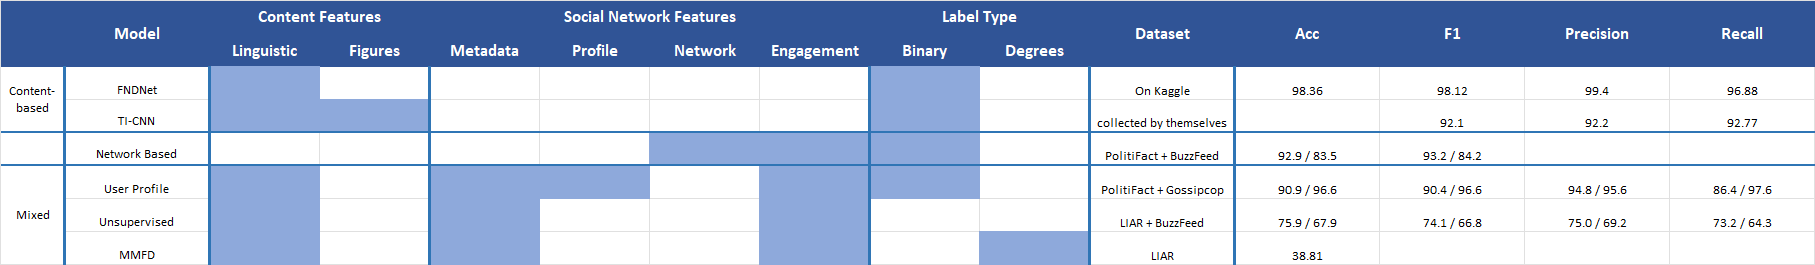
\includegraphics[width=\linewidth]{summary.png}
  \caption{A summary of mentioned models with their features, label types, datasets amd performances.}
  \Description{A table of the summarization}
\end{figure*}

\section{Methods}
As an analogous of appeared patterns, the models examined in this section will be summarized by their applied features. Specifically, the pure content-based approaches, the pure social network based approaches, and the mixture of both.

\subsection{Pure Content Based}
Both FNDNet and TI-CNN use only the content to detect fake news, while FNDNet uses only textual information and TI-CNN combines textual with images \cite{FNDNet,yang2018ti}. However, the datasets used by both of them are unclear.

\subsubsection{FNDNet}
FNDNet \cite{FNDNet} is a machine learning approach which extracted the features from the raw data by utilizeing an exist natural language processing method, GloVe \cite{glove}. GloVe calculates the clossness of two words in context and is storded as a matrix, $\mathcal{Z}$. $\mathcal{Z}$ is then passed through sevral steps of CNN with ReLu as activate function and pooling, but lack of explanations. The authors provide an accuracy of 98\% of this model by applying to a dataset on Kaggle. This value, however, would be less believable due to the simultaneously high performance of the baselines, but it would also be because of the importance of GloVe.

\subsubsection{TI-CNN}
Different from FNDNet which considers only the text content, TI-CNN includes both the textual content and the attached images \cite{yang2018ti}. According to the authors, the statistical features of words, sentences, and images are proved to distinguish from real news to fake news, which forms the dataset $\mathcal{X}$. Then $\mathcal{X}$ is passed through CNNs to form the training data $\mathcal{Z}$. Finally, the neural network $\mathcal{Z}$ is trained with a back-propagation algorithm. The dataset used in this paper is collected by the authors themselves because of the special requirement of image containing. They tested the effectivity of their model by applying baseline models on the same datasets, and the results reliably proved the importance of attached images.

\subsection{Pure Social Network Based}
Based on my research, only one model is purely network based, which is developed by Zhou et al. (2019) \cite{NetworkBased}. In their article, four different patterns of fake news are carefully analyzed. They first use CNN to extract the considered features from raw data and then use the random forest as the training model. In order to analyze the importance of each pattern, they used different combinations of features on two benchmark datasets, PolitiFact and BuzzFeed. Based on their results, the spreader pattern is the most important part followed by the user engagement.


\subsection{Mixture}
Combing both feature domains is a wise decision and is more commonly used because it provides more variable combinations and may avoid being blinded by one of them. However, the dimension of features increases significantly compared to the previous methods, so a more effective method to extract features and reduce the dimension is relatively important. Three different approaches will be examined in this part.

\subsubsection{User Profiles}
The importance of user profiles is analyzed by Shu et al. (2019) \cite{UserProfile}. They used CNN to extract implicit user profiles, including location, profile images, and political basis. The datasets used in this paper are two benchmark datasets, PolitiFact and Gossipcop. They proved the importance of user profiles by comparing the results using only writing style, only content correctness, only user profiles, and a mixture. The results show that even only using user profiles as the features, the result outperforms the linguistic features, while the mixture further improves the performance.

\subsubsection{Unsupervised Detection Model}
An unsupervised framework is provided by Yang et al. (2019) \cite{Unsupervised}. This article intends to solve the difficulty in collecting reliably labeled datasets. An unsupervised model may also quickly react to updated news because no prior requirement of labeling the data points. This framework, however, is stated only with statistical equations which diminishes the interpretability. In their approach, user credibilities are calculated based on their metadata and engagements. They tested the effectivity of this model with user credibilities and linguistic patterns as the features on two benchmark datasets, LIAR + BuzzFeed. The performance shows an accuracy of around 70\%. 

\subsubsection{MMFD}
Multi-source Muilti-class Fake News Detection (MMFD) \cite{MMFD} allows the consideration of more different patterns. It also generates the degress of fakeness as the labels though CNN combining with LSTM. According to the authors, one challenge of their model is the diffference in dimentions of each applied source. They also used word2vec to transform the contents into matrices. They trained their model by Stochastic Gradient Descent (SGD) with the loss function:
\begin{equation*}
\mathcal{L} = \lambda\times \text{CrossEntropy} +(1-\lambda)(\beta_1\epsilon^{intra} + \beta_2\epsilon^{inter})
\end{equation*}
where $\lambda$ is the regularization parameter, $\epsilon^{intra}$ is the intra-class distance, $\epsilon^{inter}$ is the inter-class distance, and $\beta_1$, $\beta_2$ are hyper-parameters. They used LIAR as their dataset, and the result shows an accuracy lower than 40\%. This low performance probably due to the difficulty of labeling the data points.

\section{Discussion}
Figure 1 shows the general information of each model. As can be seen, various datasets are used, which increases the difficulty of comparison, so creating a more generally acceptable benchmark dataset is important. Notice that FNDNet obtains an incredibly high accuracy. By further analyzing their dataset, two problems appear: (i) the lack of data points and (ii) the balanced numbers of real news and fake news. In the real world, fake news is hard to collect compared with real news, leading to fewer in number. Also noticed that the network based approach and user profiles shared the same dataset, PolitiFact. Thus, by comparing their results, we can see that the network based approach outperformed even without content based features. This high performance convincingly proves the importance of network features in fake news detection. We can also observe that the unsupervised model performs worse than supervised models, except MMFD which obtained an extremely low accuracy. As MMFD uses both features, this accuracy should not cause by the feature selection, but by their calculated labels. Their approach fails in classifying the data points into multiple classes, but if a more reliable algorithm for calculating the degree of fakeness is developed, then the performance of this model may be improved. Another interesting finding is that all the models used CNN to extract features or to train the datasets which show the degree of appreciation of CNN in this topic. Other approaches, such as RNN, are also powerful but not discussed in this survey, so further research will continuously investigate novel approaches. 


\section{Conclusion}
The most common challenge in this topic is that the users who create fake news deliberately mix real news with artificial information to increase credibility, so models may be blinded if only considering the content. Thus, a consideration of social network based features is important. Hence, due to the previous discussion, the network patterns are significantly effective which should be included in developing other approaches. Also, some patterns mentioned in this survey may not be applied to the dataset with Covid-19 news. Specifically, the images in Covid-19 news notably differ to the ones in the news of the 2016 presidential election. Thus, to determine whether or not to use image features in Covid-19 datasets, more research on the patterns of fake news is required. Moreover, the lack of benchmark datasets of Covid-19 news is another primary problem. These listed problems are the future research goals.

\bibliographystyle{ACM-Reference-Format}
\bibliography{ref}

\end{document}
